\documentclass[../../main.tex]{subfiles}


\begin{document}

\subsection*{(a)}
After selecting the three specified attributes, normalization by Z-transformation is done. The result is multiplied so it can be fed to all k-means clusterers at once. For each clustering we set the necessary 'k' and 'max runs' and select the 'add as label' checkbox so the cluster labels are added as a new column. To use the unscaled dataset as a model we first reverse the Z-transformation by De-Normalizing and then apply it to the clustered data.\\  
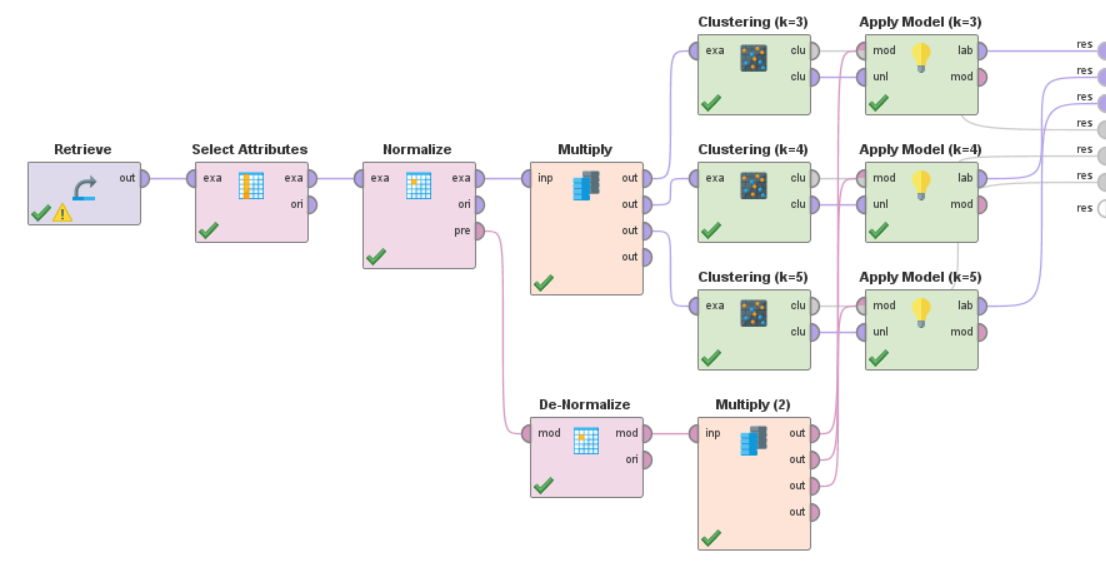
\includegraphics[width=\textwidth]{img/QUESTION_3a_PROCESS.png}

The following graphics show the clustering results for the Requested Amount on the x-Axis mapped against the Throughput times on the y-Axis (with high Jitter for better visualization of regions). Additionally, Number of Offers was chosen to determine the size of each dot on the scatter plot to visualize all 3 dimensions at once. Over all $k\in\{3,4,5\}$ there are a few similar clusters:
\begin{itemize}
\item One that is characterized best by its high Requested Amounts (mostly $>20k$) and Throughput times of mostly under 40 days.
\item One that is characterized by its generally lower Requested Amounts of mostly $<40k$ and Throughput times of mostly over 20 days. It also includes mostly larger Numbers of Offers. There is a little ambiguity however, for example because k=3 doesn't have a great resolution and clusters together more generously. For higher case the opposite is true, so some cases from this cluster fall to a new cluster.
\item Then there are clusters that are generally $<40k$ in Requested Amounts and with Throughput Times of mostly under 40 days. These clusters change the most for different k and also frequently intersect with other clusters in the x and y dimension, especially for lower k.\\
\end{itemize}
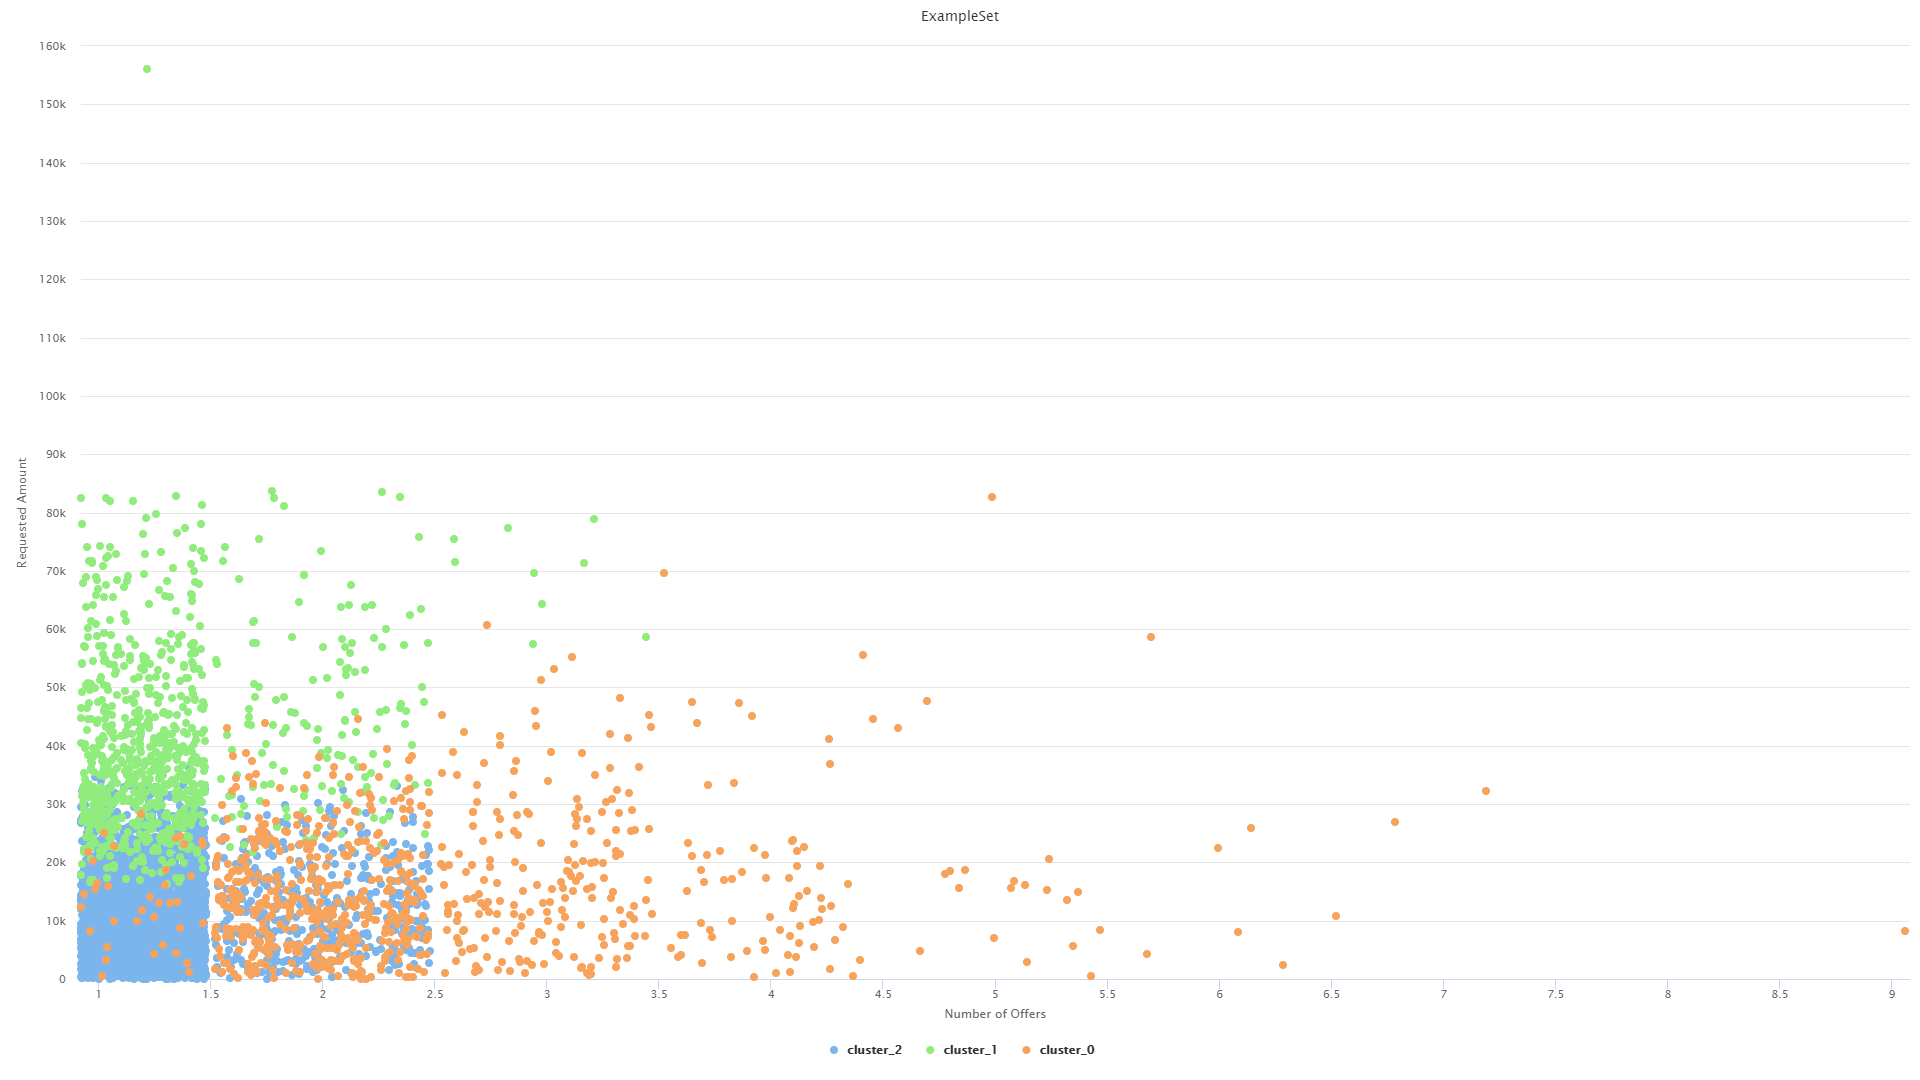
\includegraphics[width=\textwidth]{img/QUESTION_3a_kmeans_3_offers_amount.png}
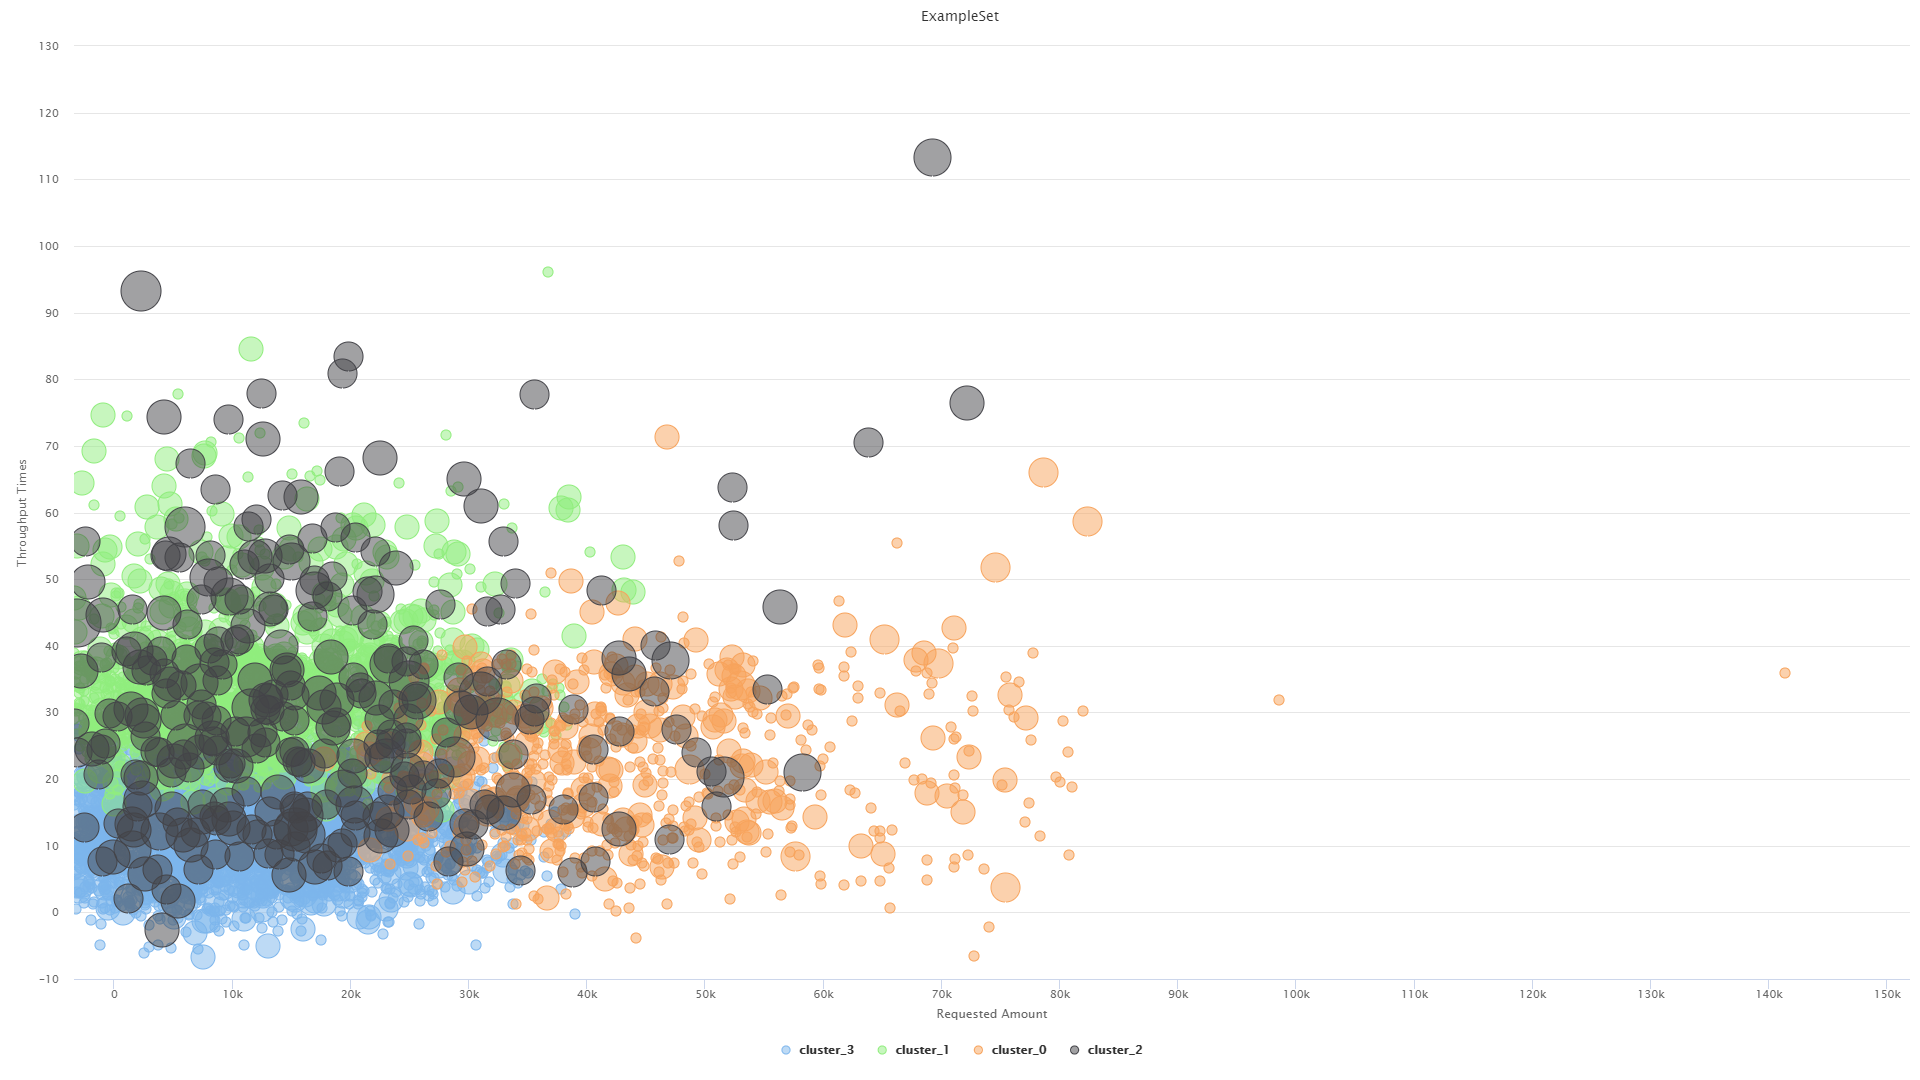
\includegraphics[width=\textwidth]{img/QUESTION_3a_kmeans_4_offers_amount.png}
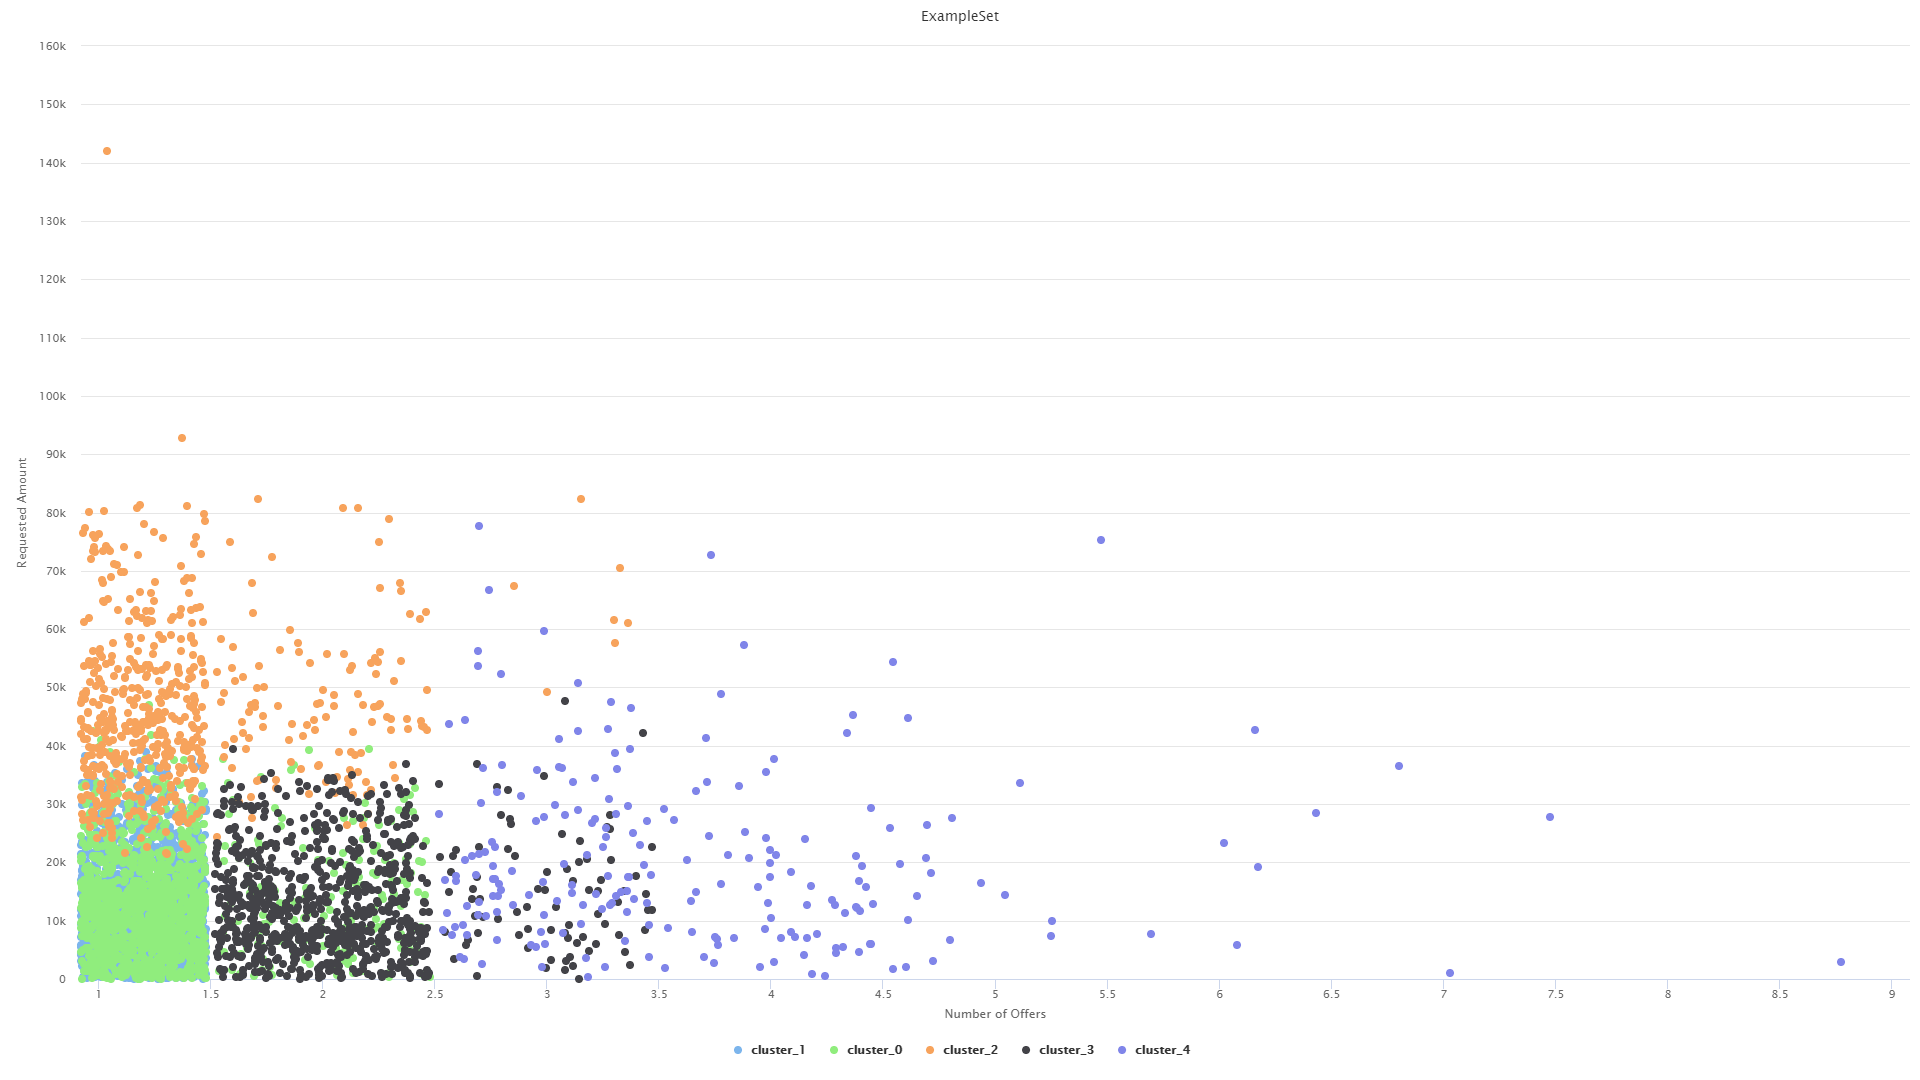
\includegraphics[width=\textwidth]{img/QUESTION_3a_kmeans_5_offers_amount.png}

As mentioned above, k=3 has a very low 'resolution' which makes it hard to differentiate between clusters. For this reason k=4 or k=5 are more suitable to distinguish clusters. Especially for k=5 it is easy to see which traits define a cluster and therefore an intuitive discription of what applications belong to it become easier. 
Even visually these applications are very distinguishable because they are always very similar in at least 2 parameters.\\
One could argue that a lower amount of clusters is advantageous because there aren't so many different types of loan applications to consider in management ($\Rightarrow$ maybe less bureaucracy), however we cannot judge this well with our knowledge and because k=5 is not that large of a number we choose it as the most suitable one.\\ 

The value of cluster centroids are displayed in the 3 tables below:\\
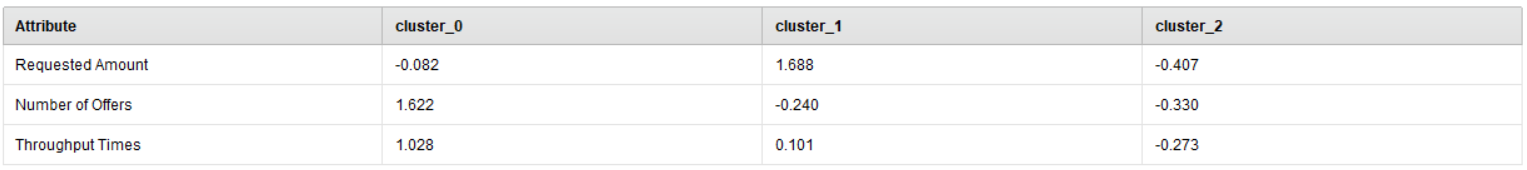
\includegraphics[width=\textwidth]{img/QUESTION_3a_kmeans_3_centroids.png}
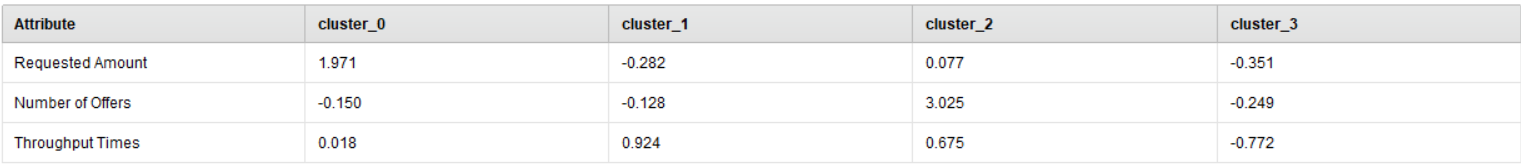
\includegraphics[width=\textwidth]{img/QUESTION_3a_kmeans_4_centroids.png}
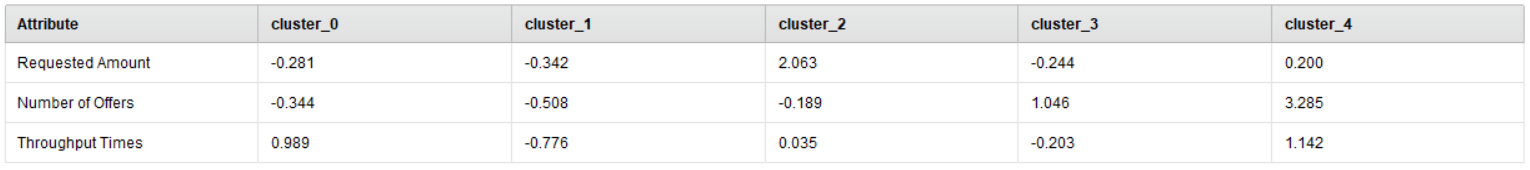
\includegraphics[width=\textwidth]{img/QUESTION_3a_kmeans_5_centroids.png}

The number of applications in each cluster is displayed below:\\
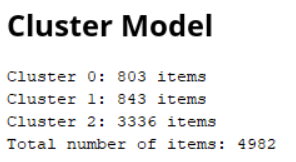
\includegraphics[width=\textwidth/3]{img/QUESTION_3a_kmeans_3_cluster_sizes.png}
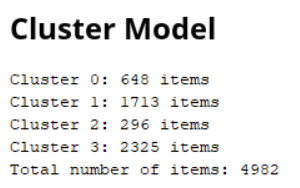
\includegraphics[width=\textwidth/3]{img/QUESTION_3a_kmeans_4_cluster_sizes.png}
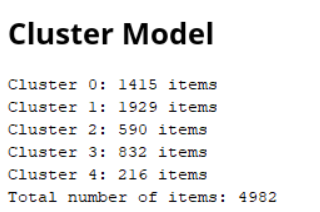
\includegraphics[width=\textwidth/3]{img/QUESTION_3a_kmeans_5_cluster_sizes.png}

\subsection*{(b)}
1. 1929 of our 4982 applications ($38.7\%$) were for amounts of less than 40k and were handled within a month with just one offer.\\
2. Our large amount applications ($>30k$) were mostly handled within a month.\\
3. The applications with longer throughput times generally had larger numbers of offers

\end{document}